\begin{center}
	\begin{tabular}{M{9.25cm}M{8.75cm}}
		\textbf{TRƯỜNG THCS-THPT NGUYỄN KHUYẾN}& \textbf{ÔN TẬP KIỂM TRA CUỐI HỌC KÌ I}\\
		\textbf{MÃ ĐỀ: 002}& \textbf{Bài thi môn: VẬT LÝ 10}\\
		\textit{(Đề thi có 04 trang)}& \textit{Thời gian làm bài: 45 phút, không kể phát đề}
		
		\noindent\rule{4cm}{0.8pt} \\
	\end{tabular}
\end{center}
\setcounter{section}{0}
\section{Câu trắc nghiệm nhiều phương án lựa chọn}
\textit{Thí sinh trả lời từ câu 1 đến câu 18. Mỗi câu hỏi thí sinh chọn một phương án}
\setcounter{ex}{0}
\Opensolutionfile{ans}[ans/D10-CK1-002-TN]
% ===================================================================
\begin{ex}
	Người ta thường dùng quãng đường đi được trong cùng một đơn vị thời gian để xác định độ nhanh, chậm của chuyển động. Đại lượng này gọi là
	\choice
	{vận tốc trung bình}
	{\True tốc độ trung bình}
	{tốc độ tức thời}
	{vận tốc tức thời}
	\loigiai{}
\end{ex}
% ===================================================================
\begin{ex}
	Điều nào sau đây là \textbf{sai} khi nói về trọng lực?
	\choice
	{Trọng lực được xác định bởi biểu thức $\vec{P}=m\cdot\vec{g}$}
	{Điểm đặt của trọng lực là trọng tâm của vật}
	{\True Trọng lực có độ lớn tỉ lệ nghịch với khối lượng của vật}
	{Trọng lực là lực hút của Trái Đất tác dụng lên vật}
	\loigiai{}
\end{ex}
% ===================================================================
\begin{ex}
Trong một cơn giông, một cành cây bị gãy và bay trúng vào một cửa kính, làm vỡ kính. Chọn nhận xét đúng.	
	\choice
	{Lực của cành cây tác dụng lên tấm kính lớn hơn lực của tấm kính tác dụng vào cành cây}
	{\True Lực của cành cây tác dụng lên tấm kính có độ lớn bằng lực của tấm kính tác dụng vào cành cây}
	{Lực của cành cây tác dụng lên tấm kính nhỏ hơn lực của tấm kính tác dụng vào cành cây}
	{Cành cây không tương tác với tấm kính khi làm vỡ kính}
	\loigiai{}
\end{ex}
% ===================================================================
\begin{ex}
Chỉ ra phát biểu \textbf{sai}.\\
Độ lớn của lực ma sát trượt	
	\choice
	{\True phụ thuộc vào diện tích tiếp xúc của vật}
	{không phụ thuộc vào tốc độ của vật}
	{tỉ lệ với độ lớn của áp lực}
	{phụ thuộc vào vật liệu và tính chất của hai mặt tiếp xúc}
	\loigiai{}
\end{ex}
% ===================================================================
\begin{ex}
	Lực đẩy Archimedes phụ thuộc vào các yếu tố:
	\choice
	{trọng lượng riêng của chất lỏng và thể tích của vật}
	{trọng lượng của chất lỏng và thể tích của phần chất lỏng bị vật chiếm chỗ}
	{\True trọng lượng riêng của chất lỏng và thể tích của phần chất lỏng bị vật chiếm chỗ}
	{trọng lượng riêng của vật và thể tích của phần chất lỏng bị vật chiếm chỗ}
	\loigiai{}
\end{ex}
% ===================================================================
\begin{ex}
	Một người kéo xe hàng trên mặt sàn nằm ngang, lực tác dụng lên người để làm người chuyển động về phía trước là lực mà
	\choice
	{người tác dụng vào xe}
	{xe tác dụng vào người}
	{người tác dụng vào mặt đất}
	{\True mặt đất tác dụng vào người}
	\loigiai{}
\end{ex}
% ===================================================================
\begin{ex}
Khi vật đang chuyển động thẳng và đổi chiều chuyển động thì đại lượng nào sau đây đổi dấu?	
	\choice
	{Tốc độ trung bình và vận tốc trung bình}
	{Tốc độ tức thời}
	{\True Độ dịch chuyển và vận tốc}
	{Quãng đường và độ dịch chuyển}
	\loigiai{}
\end{ex}
% ===================================================================
\begin{ex}
	Câu nào sau đây là \textbf{sai} khi nói về lực căng dây?
	\choice
	{Lực căng dây có bản chất là lực đàn hồi}
	{Lực căng dây có điểm đặt là điểm mà đầu dây tiếp xúc với vật}
	{Lực căng có phương trùng với chính sợi dây, chiều hướng từ hai đầu vào phần giữa của sợi dây}
	{\True Lực căng có thể là lực kéo hoặc lực nén}
	\loigiai{}
\end{ex}
% ===================================================================
\begin{ex}
	Các giọt mưa rơi thẳng đứng với tốc độ $\SI{6}{\kilo\meter/\hour}$. Một người đi bộ trên đường thẳng nằm ngang với tốc độ $\SI{8}{\kilo\meter/\hour}$. Vận tốc tương đổi của giọt mưa đối với người có độ lớn là
	\choice
	{$\SI{7}{\kilo\meter/\hour}$}
	{\True $\SI{10}{\kilo\meter/\hour}$}
	{$\SI{14}{\kilo\meter/\hour}$}
	{$\SI{2}{\kilo\meter/\hour}$}
	\loigiai{}
\end{ex}
% ===================================================================
\begin{ex}
	Một xe có khối lượng $m=\SI{5}{\text{tấn}}$ đang đứng yên trên mặt phẳng nghiêng $\SI{30}{\degree}$ so với phương ngang. Độ lớn của lực ma sát tác dụng lên xe
	\choice
	{lớn hơn trọng lượng của xe}
	{bằng trọng lượng của xe}
	{bằng độ lớn của thành phần trọng lực vuông góc với mặt phẳng nghiêng}
	{\True bằng độ lớn của thành phần trọng lực song song với mặt phẳng nghiêng}
	\loigiai{}
\end{ex}
% ===================================================================
\begin{ex}
Một thỏi nhôm và một thỏi thép có thể tích bằng nhau cùng được nhúng chìm trong nước. Nhận xét nào sau đây là \textbf{đúng}?	
	\choice
	{Thỏi nào chìm sâu hơn thì lực đẩy Archimedes tác dụng lên thỏi đó lớn hơn}
	{\True Hai thỏi nhôm và thép đều chịu tác dụng của lực đẩy Archimedes như nhau vì chúng chiếm thể tích trong nước như nhau}
	{Hai thỏi nhôm và thép đều chịu tác dụng của lực đẩy Archimedes như nhau vì chúng cùng được nhúng trong nước}
	{Thép có trọng lượng riêng lớn hơn nhôm nên thỏi thép chịu tác dụng của lực đẩy Archimedes lớn hơn}
	\loigiai{}
\end{ex}

% ===================================================================
\begin{ex}
	Lực hãm không đổi có độ lớn $F$ tác dụng vào vật khối lượng $m$ đang chuyển động với vận tốc ban đầu $v$. Sau thời gian $t$ bao lâu thì vật đó đứng yên?
	\choice
	{$t=\dfrac{vF}{m}$}
	{\True $t=\dfrac{mv}{F}$}
	{$t=\dfrac{F}{mv}$}
	{$t=\dfrac{v}{mF}$}
	\loigiai{}
\end{ex}
% ===================================================================
\begin{ex}
	Một xe ô tô đang chạy trên đường thẳng nằm ngang với tốc độ $v_0=\SI{72}{\kilo\meter/\hour}$ thì tắt máy. Quãng đường ô tô đi được từ lúc tắt máy đến khi dừng hẳn là $\SI{40}{\meter}$. Lấy gia tốc trọng trường $g=\SI{10}{\meter/\second^2}$. Hệ số ma sát giữa bánh xe và mặt đường là
	\choice
	{\True $\mu=0,5$}
	{$\mu=0,4$}
	{$\mu=0,3$}
	{$\mu=0,6$}
	\loigiai{}
\end{ex}
% ===================================================================
\begin{ex}
Một vật có khối lượng $\SI{3}{\kilogram}$ đang chuyển động thẳng đều với vận tốc $v_0=\SI{2}{\meter/\second}$ thì chịu tác dụng của một lực $\SI{9}{\newton}$ cùng chiều với $\vec{v}_0$. Vật sẽ chuyển động $\SI{10}{\meter}$ tiếp theo trong thời gian	
	\choice
	{\True $\SI{2}{\second}$}
	{$\SI{3}{\second}$}
	{$\SI{4}{\second}$}
	{$\SI{5}{\second}$}
	\loigiai{}
\end{ex}
% ===================================================================
\begin{ex}
	Thể tích của một miếng sắt là $\SI{2}{\deci\meter^3}$. Cho khối lượng riêng của nước là $\SI{1000}{\kilogram/\meter^3}$. Lấy $g=\SI{9.8}{\meter/\second^2}$. Lực đẩy tác dụng lên miếng sắt khi nhúng chìm trong nước có giá trị là
		\choice
	{$\SI{25}{\newton}$}
	{$\SI{20}{\newton}$}
	{\True $\SI{19.6}{\newton}$}
	{$\SI{19600}{\newton}$}
	\loigiai{}
\end{ex}
% ===================================================================
\begin{ex}
\immini{Một chất điểm chịu tác dụng của ba lực $\vec{F}_1$, $\vec{F}_2$, $\vec{F}_3$ có cùng độ lớn $\SI{12}{\newton}$. Biết góc tạo bởi các lực $\left(\vec{F}_1, \vec{F}_2\right)=\left(\vec{F}_2,\vec{F}_3\right)=\SI{60}{\degree}$. Hợp lực của ba lực này có độ lớn 	
\choice
{$\SI{6}{\newton}$}
{\True $\SI{24}{\newton}$}
{$\SI{10.4}{\newton}$}
{$\SI{20.8}{\newton}$}}
{\vspace{-0.5cm}\begin{tikzpicture}
		\coordinate (O) at (0,0);
		\coordinate (F1) at ($(O)+(30:2)$);
		\coordinate (F2) at ($(O)+(90:2)$);
		\coordinate (F3) at ($(O)+(150:2)$);
		\tkzMarkAngle[size=0.6cm,color=red, line width=1.2pt](F1,O,F2);
		\tkzLabelAngle[color=black,pos=1.0](F1,O,F2){$\SI{60}{\degree}$};
		\tkzMarkAngle[size=0.75cm,color=red, line width=1.2pt](F2,O,F3);
		\tkzLabelAngle[color=black,pos=1.2](F2,O,F3){$\SI{60}{\degree}$};
		\draw[-stealth, line width=1.5pt, blue] (O)--(F1);
		\draw[-stealth, line width=1.5pt, blue] (O)--(F2);
		\draw[-stealth, line width=1.5pt, blue] (O)--(F3);
		\node[above, blue] at (F1) {$\vec{F}_1$};
		\node[above, blue] at (F2) {$\vec{F}_2$};
		\node[above, blue] at (F3) {$\vec{F}_3$};
\end{tikzpicture}}
	
	\loigiai{}
\end{ex}
% ===================================================================
\begin{ex}
Vật nhỏ khối lượng $m=\SI{5}{\kilogram}$ nằm yên trên mặt phẳng ngang. Tác dụng lên vật lực kéo $F=\SI{12}{\newton}$ theo phương ngang. Lấy $g=\SI{10}{\meter/\second^2}$. Hệ số ma sát giữa vật và mặt phẳng ngang là $0,2$.	  Sau khi vật trượt được $\SI{5}{\meter}$ thì ngừng tác dụng lực. Quãng đường dài nhất vật đi từ lúc bắt đầu chuyển động là
	\choice
	{$\SI{8}{\meter}$}
	{\True $\SI{6}{\meter}$}
	{$\SI{1}{\meter}$}
	{$\SI{10}{\meter}$}
	\loigiai{}
\end{ex}
% ===================================================================
\begin{ex}
	Một sợi dây có thể treo một vật đứng yên có khối lượng tối đa là $\SI{50}{\kilogram}$ mà không bị đứt. Dùng sợi dây này để kéo một vật khác có khối lượng $\SI{45}{\kilogram}$ lên cao theo phương thẳng đứng. Lấy gia tốc trọng trường $g=\SI{10}{\meter/\second^2}$. Gia tốc lớn nhất mà vật có thể có để dây không bị đứt là
	\choice
	{\True $\SI{1.1}{\meter/\second^2}$}
	{$\SI{11.1}{\meter/\second^2}$}
	{$\SI{21.1}{\meter/\second^2}$}
	{$\SI{10.5}{\meter/\second^2}$}
	\loigiai{}
\end{ex}
\Closesolutionfile{ans}
\section{Câu trắc nghiệm đúng/sai} 
\textit{Thí sinh trả lời từ câu 1 đến câu 4. Trong mỗi ý \textbf{a)}, \textbf{b)}, \textbf{c)}, \textbf{d)} ở mỗi câu, thí sinh chọn đúng hoặc sai}
\setcounter{ex}{0}\\
\Opensolutionfile{ans}[ans/D10-CK1-002-TF]
% ===================================================================
\begin{ex}
	Một quyển sách đang được đặt nằm yên trên mặt bàn nằm ngang.	Nhận định các phát biểu sau đây:
	\choiceTF[t]
	{\True Trọng lực tác dụng lên quyển sách cũng là lực hấp dẫn do Trái Đất tác dụng lên sách}
	{Trọng lực của quyển sách và phản lực của mặt bàn tác dụng lên sách có cùng bản chất}
	{Quyển sách chịu tác dụng của lực ma sát nghỉ có phương song song với mặt bàn}
	{Trọng lực tác dụng lên sách luôn có độ lớn bằng phản lực của bàn tác dụng lên sách}
	\loigiai{}
\end{ex}

% ===================================================================
\begin{ex}
	Hai xe đồ chơi A và B chuyển động trên mặt phẳng nằm ngang với tốc độ lần lượt là $\SI{50}{\centi\meter/\second}$ và $\SI{150}{\centi\meter/\second}$. Xe B tới va chạm với xe A từ phía sau. Sau va chạm, hai xe chuyển động với cùng tốc độ $\SI{100}{\centi\meter/\second}$. Biết rằng trong suốt quá trình va chạm, các vector vận tốc không đổi hướng.
	\choiceTF[t]
	{Độ lớn lực do xe A tác dụng lên xe B lớn hơn độ lớn lực do xe B tác dụng lên xe A}
	{Xe A tác dụng lực lên xe B trước, sau đó xe B mới tác dụng lực lên xe A}
	{Gia tốc của hai xe trong quá trình va chạm là bằng nhau}
	{Khối lượng xe A lớn hơn khối lượng xe B}
	\loigiai{}
\end{ex}
% ===================================================================
\begin{ex}
	Một quả cầu đặc được làm bằng nhôm. Người ta treo quả cầu bên dưới một lực kế trong không khí, lực kế chỉ $\SI{7.1}{\newton}$. Biết khối lượng riêng của nhôm, nước và dầu lần lượt là $\rho_1=\SI{2700}{\kilogram/\meter^3}$, $\rho_2=\SI{1000}{\kilogram/\meter^3}$, $\SI{800}{\kilogram/\meter^3}$. Lấy gia tốc trọng trường $g=\SI{9.8}{\meter/\second^2}$. Thể tích khối cầu bán kính $r$ được xác định bởi $V=\dfrac{4}{3}\pi r^3$.
	\choiceTF[t]
	{\True Bán kính quả cầu nhôm là $\SI{4}{\centi\meter}$}
	{\True Nhúng quả cầu chìm trong dầu thì số chỉ lực kế là $\SI{5}{\newton}$}
	{Nếu nhúng quả cầu vào trong nước, quả cầu chỉ chìm một phần}
	{\True Để quả cầu lơ lửng trong dầu, người ta phải khoét rỗng phần bên trong của quả cầu với bán kính phần rỗng là $\SI{35.6}{\milli\meter}$}
	\loigiai{}
\end{ex}
% ===================================================================
\begin{ex}
	\immini{Một vật nhỏ có khối lượng $\SI{15}{\kilogram}$ được giữ nằm yên trên mặt phẳng nghiêng không ma sát với góc nghiêng $\SI{27}{\degree}$ so với mặt ngang bằng một sợi dây nhẹ, không dãn như hình. Lấy $g=\SI{9.8}{\meter/\second^2}$. }{\vspace{-0.5cm}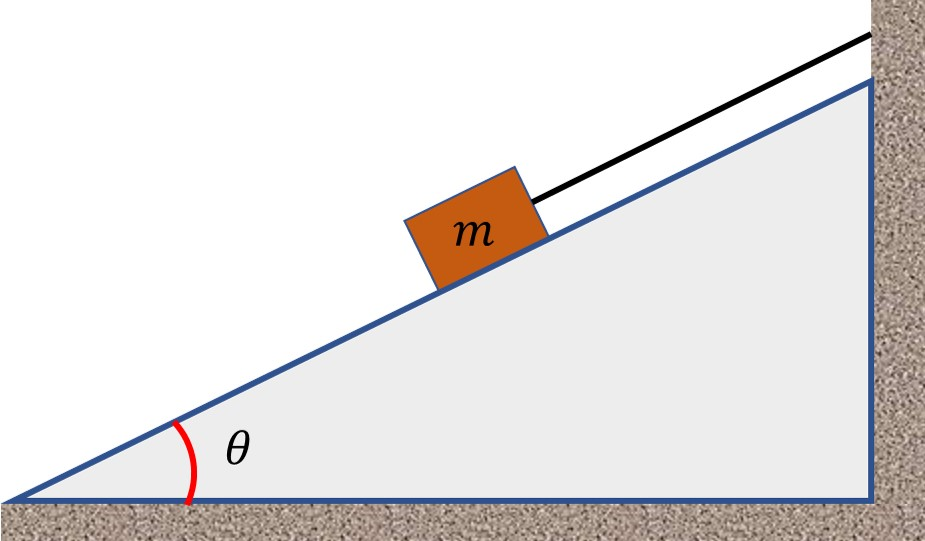
\includegraphics[scale=0.25]{figs/D10-CK1-002-1}}
	\choiceTF[t]
	{Phản lực của mặt phẳng nghiêng tác dụng lên vật cân bằng với trọng lực của vật}
	{\True Lực căng của sợi dây là $\SI{67}{\newton}$}
	{\True Khi cắt đứt dây giữ vật thì vật sẽ trượt xuống với gia tốc có độ lớn $\SI{4.4}{\meter/\second^2}$}
	{Nếu tăng góc nghiêng thì áp lực của vật lên mặt phẳng nghiêng tăng lên}
	\loigiai{2,6}
\end{ex}
\Closesolutionfile{ans}
\section{Câu trắc nghiệm trả lời ngắn} \textit{Thí sinh trả lời từ câu 1 đến câu 6}
\setcounter{ex}{0}
\Opensolutionfile{ans}[ans/D10-CK1-002-TL]
% ===============================================================
\begin{ex}
Một ô tô đang chạy với tốc độ $\SI{10}{\meter/\second}$ trên một đoạn đường thẳng thì người lái xe tăng ga cho ô tô chạy nhanh dần đều. Sau $\SI{20}{\second}$, ô tô đạt tốc độ $\SI{14}{\meter/\second}$. Tính quãng đường ô tô đi được sau $\SI{50}{\second}$ kể từ khi tăng ga theo đơn vị mét $\left(\si{\meter}\right)$.	
	\shortans[oly]{750}
	\loigiai{
		
	}
\end{ex}
% ===============================================================
\begin{ex}
\immini{Một đèn tín hiệu giao thông có trọng lượng $\SI{1.00E2}{\newton}$ được treo cố định nhờ ba sợi dây như hình bên. Hai sợi dây cáp ở trên hợp với phương ngang các góc lần lượt $\SI{37.0}{\degree}$ và $\SI{53.0}{\degree}$. Xác định độ lớn lực căng trên dây cáp $T_2$ theo đơn vị newton $\left(\si{\newton}\right)$. \textit{(Kết quả làm tròn đến chữ số hàng phần mười)}.}	
{\vspace{-0.5cm}
	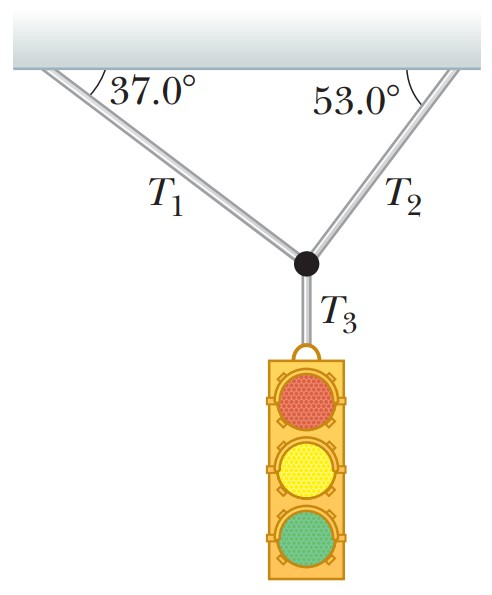
\includegraphics[scale=0.3]{figs/D10-CK1-002-4}}
	\shortans[oly]{79,9}
	\loigiai{
		
	}
\end{ex}
% ===============================================================
\begin{ex}
	\immini{Một người đẩy máy cắt cỏ có khối lượng $\SI{15}{\kilogram}$ di chuyển với một lực có độ lớn xem như không đổi bằng $\SI{80}{\newton}$ theo phương của giá đẩy như hình bên. Biết góc tạo bởi giá đẩy và phương ngang là $\SI{45}{\degree}$. Nếu từ trạng thái nghỉ, người này tác dụng lực để tăng tốc cho máy đạt tốc độ $\SI{1.2}{\meter/\second}$ trong $\SI{3}{\second}$ thì độ lớn lực ma sát trong giai đoạn này là bao nhiêu newton ($\si{\newton}$)? \textit{(Kết quả làm tròn đến chữ số hàng phần mười).}}
	{\vspace{-0.5cm}
		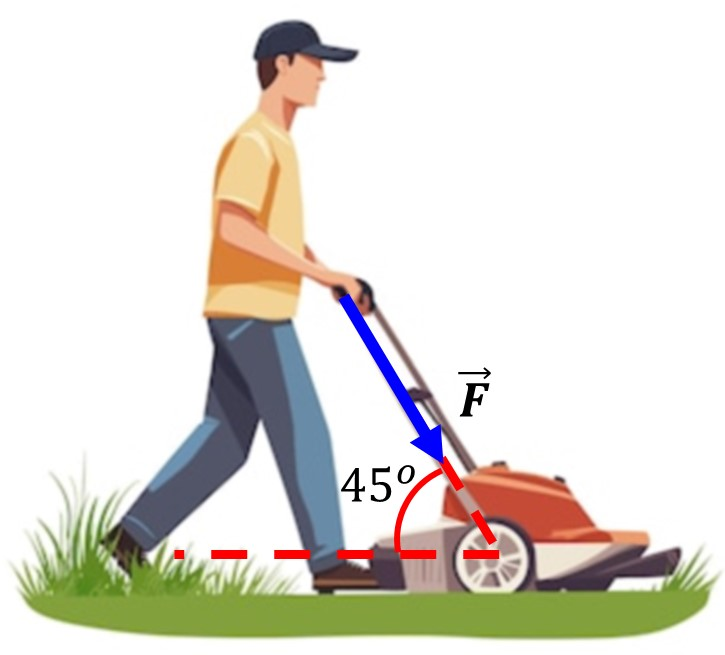
\includegraphics[scale=0.3]{figs/D10-CK1-002-3}}
	\shortans[oly]{50,6}
	\loigiai{
		
	}
\end{ex}
% ===============================================================
\begin{ex}
	\immini{Thùng hàng có trọng lượng $\SI{1000}{\newton}$ đang nằm yên trên mặt sàn nằm ngang thì chịu tác dụng bởi lực $\vec{F}$ có hướng như hình bên. Độ lớn lực $\vec{F}$ là $\SI{300}{\newton}$. Xác định tỉ số áp lực của thùng hàng lên mặt sàn trong trường hợp a và trường hợp b.	\textit{(Kết quả làm tròn đến chữ số hàng phần mười)}.}
	{\vspace{-0.5cm}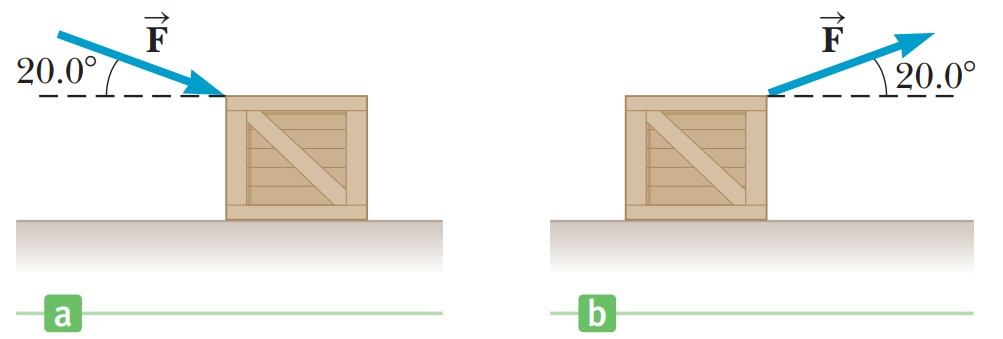
\includegraphics[scale=0.4]{figs/D10-CK1-001-4}}
	\shortans[oly]{1,2}
	\loigiai{
		
	}
\end{ex}
% ===============================================================
\begin{ex}
	\immini{Một vật nhỏ khối lượng $m=\SI{2}{\kilogram}$ đang nằm yên trên mặt bàn nằm ngang thì chịu tác dụng của lực $\vec{F}$ không đổi, theo phương song song với mặt bàn trong khoảng thời gian $\SI{8}{\second}$. Hình bên là đồ thị vận tốc thời gian của vật kể từ khi chịu tác dụng của lực $\vec{F}$. Xem như lực ma sát giữa vật và mặt bàn là không đổi trong suốt quá trình vật chuyển động. Xác định độ lớn của lực $\vec{F}$ theo đơn vị newton $\left(\si{\newton}\right)$. \textit{(Kết quả làm tròn đến chữ số hàng phần mười)}.}
	{\vspace{-0.5cm}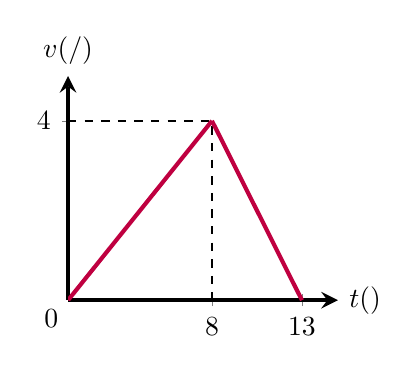
\begin{tikzpicture}  
			\begin{axis}[  ultra thick,scale=0.5,
				xmin=0,  
				xmax=15,  
				xtick={0,8,13},
				ytick={0,4},
				ymin=0,  
				ymax=5, 
				samples=300,
				axis lines=center, 
				xlabel=$\xsi{t}{\left(\si{\second}\right)}$, 		ylabel=$\xsi{v}{\left(\si{\meter/\second}\right)}$,
				every axis y label/.style={at=(current axis.above origin),anchor=south},  
				every axis x label/.style={at=(current axis.right of origin),anchor=west},  ]
				\draw[dashed, line width=0.75pt] (axis cs: 0,4)--(axis cs: 8,4)--(axis cs: 8,0);
				\addplot [line width=1.5pt, purple, smooth, domain=0:8] {0.5*x}; 
				\addplot [line width=1.5pt, purple, smooth, domain=8:13] {4-0.8*(x-8)};   
				\coordinate (O) at (axis cs: 0,0);
			\end{axis}  
			\node[below left] at (O) {0};
	\end{tikzpicture}}
	\shortans[oly]{2,6}
	\loigiai{
		
	}
\end{ex}
% ===============================================================
\begin{ex}
Lực phát động lớn nhất của một mẫu ô tô đạt được trong điều kiện thử nghiệm là $F=\SI{500}{\newton}$. Cho rằng lực cản không khí $F_c$ tác dụng lên ô tô phụ thuộc vào tốc độ của nó theo biểu thức $F_c=0,2v^2$, trong đó $v$ là tốc độ tính bằng $\si{\meter/\second}$. Xác định tốc độ khi ổn định của ô tô này trong điều kiện thử nghiệm.	
	\shortans[oly]{50}
	\loigiai{
		
	}
\end{ex}
\Closesolutionfile{ans}
\begin{center}
	\textbf{--- HẾT ---}
\end{center}